\documentclass[11pt]{article}

\usepackage[norsk]{babel}
\usepackage[utf8]{inputenc}
\usepackage{amsmath, amssymb, amsthm}
\usepackage{graphicx, float}
\usepackage{pstricks-add}


\author{Kjetil Kjeka}
\title{TTK4130 - Exercise 4}
\date{\today}


%Slik at matriser kan defineres med linjer
\makeatletter
\renewcommand*\env@matrix[1][*\c@MaxMatrixCols c]{%
  \hskip -\arraycolsep
  \let\@ifnextchar\new@ifnextchar
  \array{#1}}
\makeatother




\begin{document}
\maketitle
\section*{Problem 1}
Considering the butcher array: \\
\begin{tabular}{c|c c}
$0$ & & \\
$c_2$ & $a_{21}$ & \\ \hline
& $b_1$ & $b_2$
\end{tabular}
\subsection*{a}
The first order expansion of $k_2$ will be:
\begin{eqnarray*}
k_2 =& f(y_n + h a_{21} k_1, t_n + h c_2) &\\
=& f(y_n, t_n) + k_1 h a_{21} \frac{\partial f}{\partial y} + h c_2 \frac{\partial f}{\partial t} + O(h^2 a_{21}^2) + O(h^2 a_{21} c_2) + O(h^2 c_2^2) &\\
=& f(y_n, t_n) + k_1 h a_{21} \frac{\partial f}{\partial y} + h c_2 \frac{\partial f}{\partial t} + O(h^2) &
\end{eqnarray*}
Now assuming that $c_2 = a_{21} = K$ 
\[k_2 = f(y_n, t_n) + hK( k_1\frac{\partial f}{\partial y} + \frac{\partial f}{\partial t}) + O(h^2)\]
Since $k_1 = f(y_n, t_n)$ and $\frac{df}{dt} = f(y_n, t_n) \frac{\partial f}{\partial y} + \frac{\partial f}{\partial t}$
\[k_2 = f(y_n, t_n) + hK \frac{df}{dt} + O(h^2) \]


\subsection*{b}
For it to be order $p$, $p$ must be the smallest integer to satisfy:
\[ y_{n+1} = y_n + h f(y_n, t) + \dots + \frac{h^p}{p!} \frac{d^{p-1} f(y_n, t_n)}{dt^{p-1} + O(h^{p+1})} \]
Meaning that 
\[b_1 + b_2 = 1\] 
and 
\[b_2K = \frac{1}{2}\]
is needed for it to be of order 2.

\section*{Problem 2}
\subsection*{a}
There is no damping here, therefore eulers method wont be stable.
\begin{figure}[H]
\centering
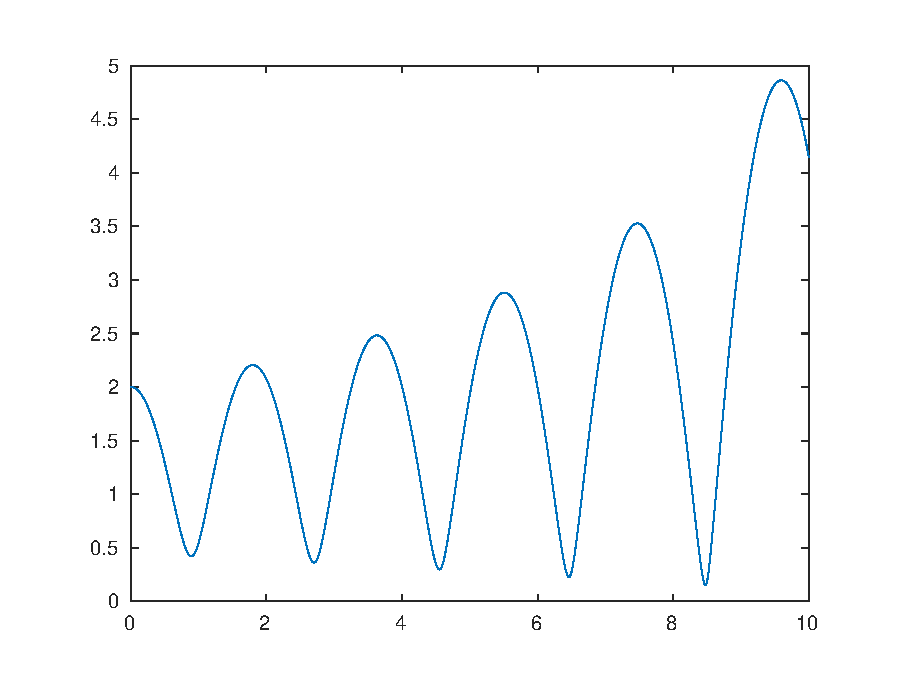
\includegraphics[width=.8\textwidth]{2a.eps}
\caption{Eulers method on maginaly stable system}
\end{figure}

\subsection*{b}
Now the simulation is stable but introduce damping such that the amplitude decreases over time.
\begin{figure}[H]
\centering
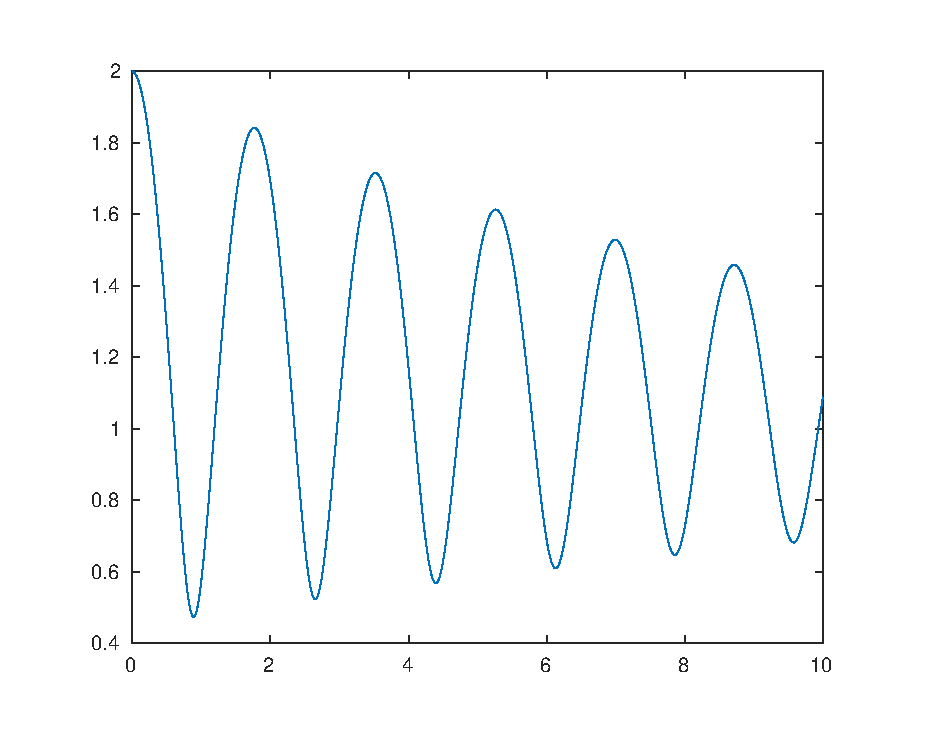
\includegraphics[width=.8\textwidth]{2b.eps}
\caption{Eulers implicit method on maginaly stable system}
\end{figure}

\subsection*{c}
Now everything seems to be physically correct.
\begin{figure}[H]
\centering
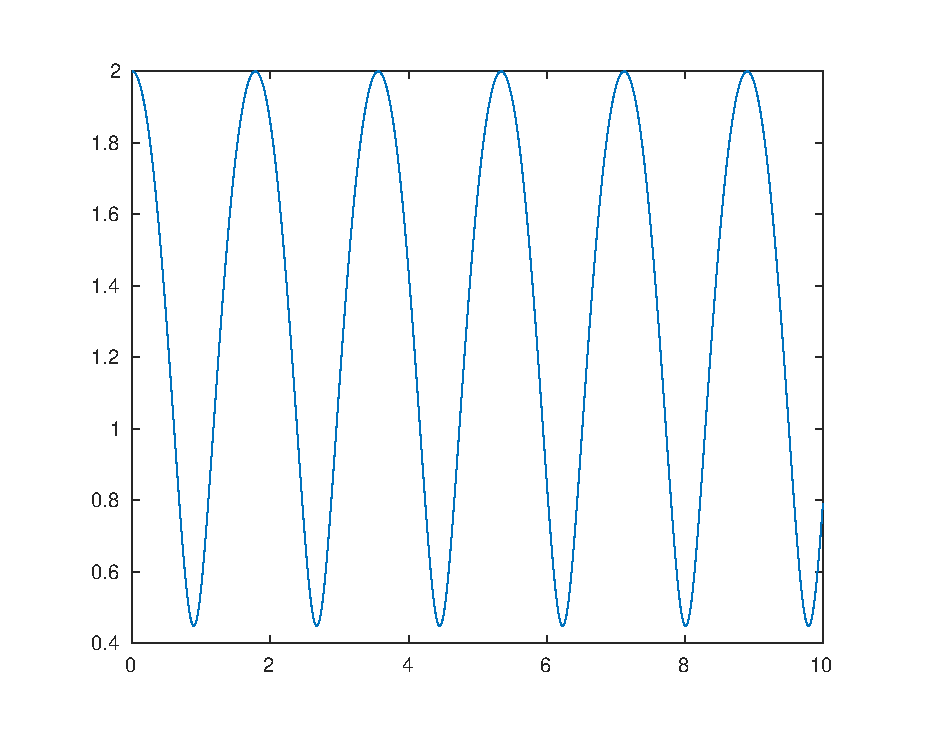
\includegraphics[width=.8\textwidth]{2c.eps}
\caption{Implicit midpoint rule on maginaly stable system}
\end{figure}

\subsection*{d}
Energy plotted for different solutions
\begin{figure}[H]
\centering
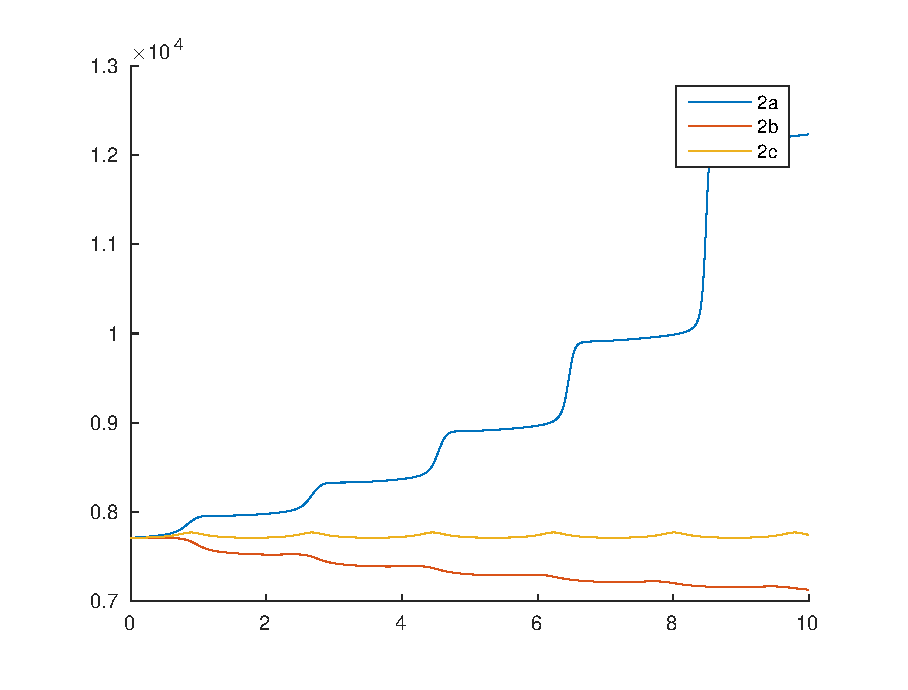
\includegraphics[width=.8\textwidth]{2d.eps}
\caption{Energy}
\end{figure}


\section*{Problem 3}
The dc motor system is given by:
\begin{eqnarray*}
L_a \frac{d i_a}{dt} &=& -R_a i_a - K_E \omega_m + u_a \\
J_m \frac{d \omega_m}{dt} &=& K_t - T_L
\end{eqnarray*}
\subsection*{a}
Let $T_L = u_a = 0$ and $K_E = K_T = K$. Using the lyapunov candidate:
\[V = \frac{1}{2} L_a i_a^2 + \frac{1}{2} J_m \omega_m\]
Which satisfies $V > 0, \forall V \not = 0$ implies that
\begin{eqnarray*}
\dot{V} &=& i_a(-R_a i_a - K \omega_m) + \omega_m(K i_a) \\
&=& -R_a i_a^2 + \omega_m i_a (K - K) \\
&=& -R_a i_a^2
\end{eqnarray*}
Which obviously satisfies $\dot{V} \leq 0$ when $R_a > 0$

\subsection*{b}
Given the input and outputs $\mathbf{u} = \begin{bmatrix} u_a \\ -T_L \end{bmatrix}$, $\mathbf{y} = \begin{bmatrix} i_a \\ \omega_m \end{bmatrix}$ and $V = \frac{1}{2} L_a i_a^2 + \frac{1}{2} J_m \omega_m^2$
\[\mathbf{u} \mathbf{y} = u_a i_a - T_L \omega_m\]
and
\begin{eqnarray*}
\dot{V} &= i_a(-R_a i_a - K \omega_m + u_a + \omega_m ( K i_a - T_L) \\
&= - R_a i_a^2 - K \omega_m i_a + i_a u_a + \omega_m K i_a - \omega_m T_L \\
&= - R_a i_a^2 + i_a u_a - \omega_m T_L \\
&= - R_a i_a^2 + \mathbf{u} \mathbf{y}^T \leq \mathbf{u} \mathbf{y}^T
\end{eqnarray*}
hence passive


\end{document}